\documentclass[12pt,a4paper]{article}
\usepackage[top=2.7cm, bottom=2cm, left=2cm, right=2cm]{geometry}
\usepackage[utf8]{inputenc}
\usepackage{CJKutf8}
\usepackage{enumitem}
\usepackage{verbatim}


%% Useful packages
\usepackage{amsmath,amssymb}
% \usepackage{subfigure}
\usepackage{graphicx,wrapfig}
\usepackage[dvipsnames,table]{xcolor}
\usepackage[table]{xcolor}
\usepackage{url}
\usepackage{setspace}
\usepackage[colorlinks=true,anchorcolor=black,linkcolor=Blue,urlcolor=RoyalBlue]{hyperref}
\usepackage[linesnumbered,ruled,vlined]{algorithm2e}
\usepackage{threeparttable}
\usepackage{arydshln}
\usepackage{tikz}
\usepackage{blindtext}
\usepackage{titlesec}
\usepackage{courier}
\usepackage{pdfpages}

\usepackage{lastpage}
\usepackage{fancyhdr}
\setlength{\headheight}{0pt}
\renewcommand{\headrulewidth}{1pt} % remove lines
\renewcommand{\footrulewidth}{0pt}
\pagestyle{fancyplain}
\fancyhf{}
\lhead{
  \textcolor{Gray}{Group 2}
}
\rhead{
  \begin{CJK}{UTF8}{bkai}
  \textcolor{Gray}{實驗結報}
  \end{CJK}
}
\lfoot{
   \textcolor{Gray}{April 29}
  }
\rfoot{
  \thepage/\pageref{LastPage}
  }

\title{\vspace{-0.5cm}
       {\bf \textcolor{black}{{\LARGE 
       \begin{CJK}{UTF8}{bkai}
       實驗物理學(二)\\
       \vspace{6pt}
        實驗報告\\
       % \vspace{60pt}
       % Fundamental Python\\
       % \vspace{6pt}
       % Basic Usage of Python
       \end{CJK}
       }}
       }
       }
\author{}
\date{}

\begin{document}
\begin{CJK}{UTF8}{bkai}

\maketitle
\thispagestyle{empty}

\vspace{10cm}
\begin{center}
{\bf \LARGE \vspace{-11cm} Fundamental Python\\
\vspace{0.25cm} Chi-square fitting - 1}\\
\vspace{13cm}
{\large Group 2}\\ \vspace{12pt}
{\large \makebox[3em][s]{洪\hspace{\fill}瑜} B125090009}\\ \vspace{6pt}
{\large \makebox[3em][s]{黃巧涵}  B122030003}\\ \vspace{6pt}
{\large \makebox[3em][s]{洪懌平} B102030019}\\ \vspace{12pt}
{\large 2025/04/29}\\
\end{center}

\clearpage
%--------------------------------------------------------------%
\vspace{2cm}
\begin{center}
{\large\bf\sc 摘要}
\end{center}

這次實驗探討了least-square fitting與chi-square fitting在數據具有非均勻不確定度時的差異,以及討論自由度對$\chi^2$分布趨勢的影響。其中Practice 1調整了資料集內不同區段的誤差大小,模擬非均勻不確定度的情況。根據擬合結果可以看出,當數據具有不均勻的誤差, chi-square fitting能夠透過調整權重產生更準確的結果,並且chi-square fitting的reduced $\chi^2$($\approx$0.061)比least square fitting的reduced $\chi^2$($\approx$0.056)更接近理論值1,代表chi-square fitting能更準確地描述資料分布之特性。透過Practice 2的隨機數據分析可以看出,自由度增加會使卡方分布趨於對稱,並且平均值會接近自由度數值,與理論相符合。本次實驗能對數據擬合方法選擇有更深刻的認識,也進一步了解$\chi^2$值與自由度之間的關聯,有助於日後處理、分析實驗數據。


\section{前言}
\hfill

% 這次實驗主要訓練正確擬合測量數據並評估誤差大小等技能。由於真實數據存在不確定性,因此透過實驗,練習如何考慮誤差,並找出最合適的擬合方法。本次實驗用到了least-square fitting 和 chi-square fitting等擬合方法。Practice 1先是模擬一組線性資料,並在x=4到x=7之區間加入較大的誤差後進行擬合與比較;Practice 2則模擬出多組高斯分布隨機資料,計算$\chi^2$值,並畫出$\chi^2$分布直方圖,比對理論的chi-square distribution,驗證自由度的影響。

\begin{itemize}
    \item Least-square fitting and Chi-square fitting:\\
    Least-square fitting為最小化殘差平方和$S$
    \begin{equation}
        S = \sum^{N}_{i=1}\left(y_i-F(x_i)\right)
    \end{equation}
    where $y_i$ is the data of the experiments, $F(x_i)$ is the model with given parameters $x_i$, and $N$ is the data size.\\
    而Chi-square fitting引入個別數據點的不確定度,為最小化加權平方和
    \begin{equation}
        \chi^2 = \sum^{N}_{i}\left(\frac{y_i-F(x_i)}{\sigma_i}\right)^2
    \end{equation}
    where $y_i$ is the data of the experiments, $F(x_i)$ is the model with given parameters $x_i$, $\sigma_i$ is the uncertainty of the experiment, and $N$ is the data size.
    \item Reduced $\chi^2$ ($\chi_{\nu}^2$):\\
    主要用於評估擬合的合理性
    \begin{equation}
        \chi_{\nu}^{2} = \frac{\chi^2}{\nu}
    \end{equation}
    其中$\nu=N-p$,$N$為資料點數,$p$為擬合參數數量
    \item Chi-square distribution and probability density function (PDF):\\
    Chi-square distribution能用來描述獨立標準常態分布變數平方和的分布情形。在資料擬合中,Chi-Square值用來衡量模型與觀測數據的吻合程度
    Probability Density Function (PDF) 是描述連續隨機變數在某個數值附近出現的機率密度有多大的函數。透過比較實做出chi-square 值之直方圖與理論的PDF值,我們可以確認實際數值是否符合預期。
    For a chi-square distribution with $k$ degrees of freedom, the PDF is 
    \begin{equation}\label{eq:pdf}
        f(x; k) = \frac{1}{2^k\Gamma(k/2)}x^{k/2-1}e^{-x/2}, \, x>0
    \end{equation}
    where $\Gamma$ is the gamma function. When $k\rightarrow\infty$, the PDF approaches a normal distribution.
\end{itemize}


\clearpage
\section{實驗步驟}

\subsection{Practice 1}
\hfill

\begin{enumerate}
    \item Generate 20 sets of data points defined by a function \( y = ax + b + \text{noise} \) with \texttt{x = np.linspace(1, 10, 10)}.
    \begin{figure}[h]
        \centering
        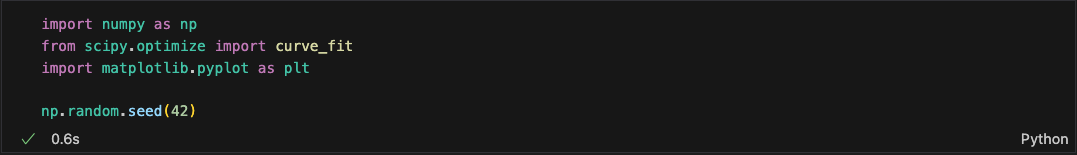
\includegraphics[width=1\linewidth]{figures/code/code_1_1.png}
        \caption{Import packages and fix the random seed to 42}
        \label{fig:code_1_1}
    \end{figure}
    \begin{figure}[h]
        \centering
        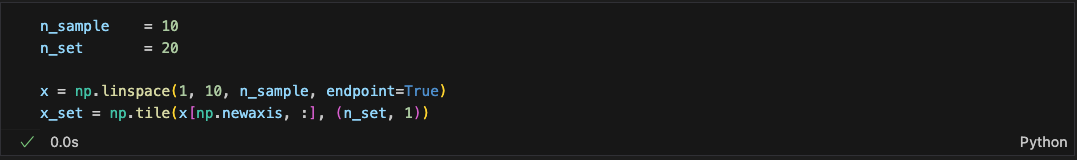
\includegraphics[width=1\linewidth]{figures/code/code_1_2.png}
        \caption{Initialize $x$}
        \label{fig:code_1_2}
    \end{figure}
    \item The noise is sampled from a normal distribution with mean = 0 and standard deviation = $\sigma_0 = 3$.
    \begin{figure}[h]
        \centering
        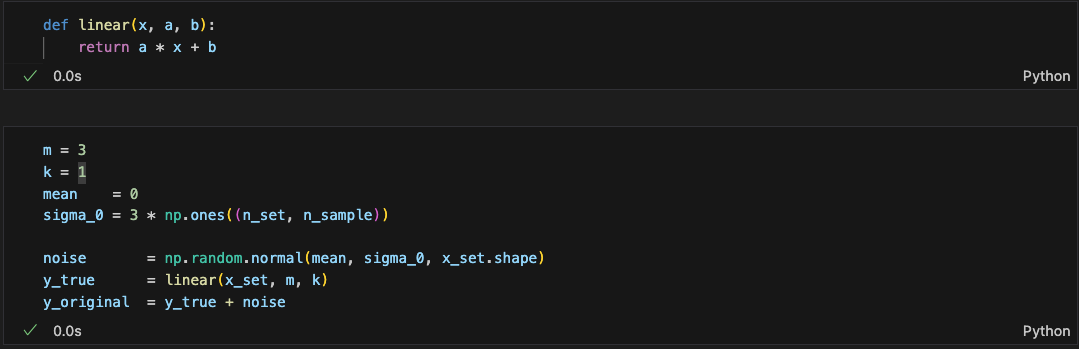
\includegraphics[width=1\linewidth]{figures/code/code_1_3.png}
        \caption{Initialize original $y$}
        \label{fig:code_1_3}
    \end{figure}
    \clearpage
    \item Change the \(\sigma_0\) of \( y \) at \( x = 4, 5, 6, 7 \) to \(\sigma_0 = 10\).
    \begin{figure}[h]
        \centering
        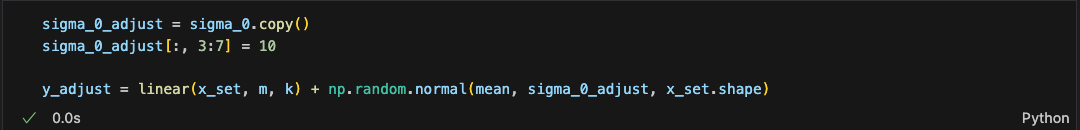
\includegraphics[width=1\linewidth]{figures/code/code_1_3_2.png}
        \caption{Adjust the $\sigma_0$ of $y$ at  $x = 4, 5, 6, 7 $}
        \label{fig:code_1_3_2}
    \end{figure}
    \item You might see that the deviation of the data points at these \( x \) values is larger than the others.
    \item Get the \emph{mean} and \emph{standard deviation} of the data points (mean value of \( y \) might be close to \( a \ast x + b \)).
    \begin{figure}[h]
        \centering
        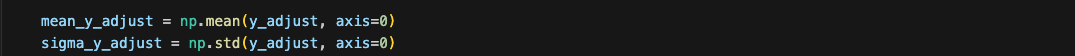
\includegraphics[width=1\linewidth]{figures/code/code_1_4.png}
        \caption{Get the \emph{mean} and \emph{standard deviation} of the data points}
        \label{fig:code_1_4}
    \end{figure}
    \item Fit these mean values of \( y \) with the function \( y = a \ast x + b \) using \texttt{curve\_fit}.
    \item Compare the difference between the least-square fitting method and the chi-square fitting method by calculating the \(\chi^2\) value.
    \begin{figure}[h]
        \centering
        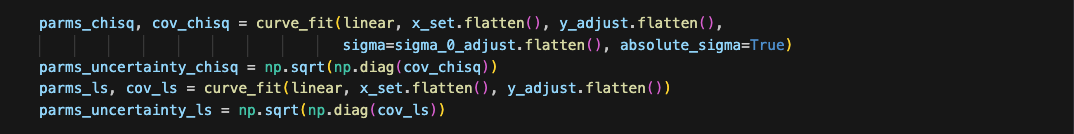
\includegraphics[width=1\linewidth]{figures/code/code_1_6.png}
        \caption{Fit these mean values of $y $ with the linear function and }
        \label{fig:code_1_6}
    \end{figure}
\end{enumerate}

\clearpage
\subsection{Practice 2}
\hfill

\begin{enumerate}
    \item Generate a 1-d array with 500 elements, each element is sampled from a normal distribution with mean = 0 and standard deviation = 1.
    \begin{figure}[h]
        \centering
        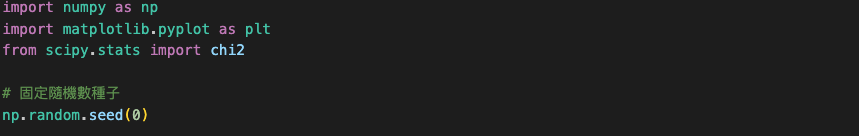
\includegraphics[width=1\linewidth]{figures/code/code_2_1.png}
        \caption{Import packages and fix the random seed to 42}
        \label{fig:code_2_1}
    \end{figure}
    \item Calculate the chi-square value of each data point:
    $\text{chisq} = \frac{(\text{data\_point} - \mu)^2}{\sigma}$
    You'll find out \(\sigma \approx 1, \mu \approx 0\). (Note that \texttt{len(chisqr)} = 500 in this case. You might feel confused about the definition of chisqr here, but just accept it for now. You can think about what it probably means in the fitting process you've done before.)
    
    \begin{figure}[h]
        \centering
        
\includegraphics[width=1\linewidth]{figures/code/code_2_2.png}\\
        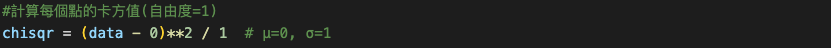
\includegraphics[width=1\linewidth]{figures/code/code_2_3.png}
        \caption{Initialize 500 elements and calculate the chi-square value.}
        \label{fig:code_2_2and3}
    \end{figure}
    \item Plot the histogram of these chi-square values.
    \item Compare the histogram with the chi-square distribution with degree of freedom = 1.
    \begin{figure}[h]
        \centering
        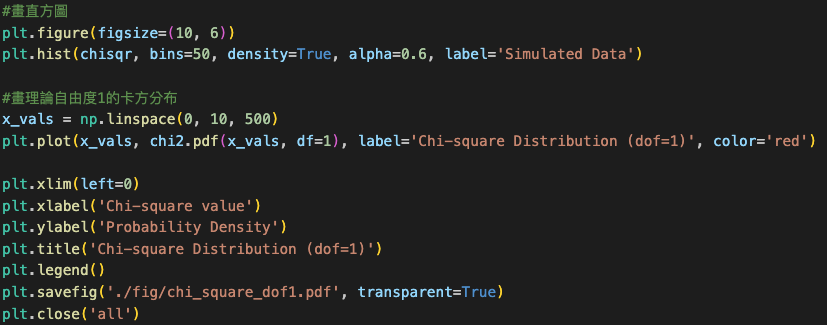
\includegraphics[width=1\linewidth]{figures/code/code_2_4.png}
        \caption{Compare the histogram with the chi-square distribution with degree of freedom = 1.}
        \label{fig:code_2_4}
    \end{figure}
    \clearpage
    \item Create several (2 to 10) 1-d arrays similar to the ones above, each array containing 500 elements sampled from a normal distribution with mean = 0 and standard deviation = 1. Then, calculate the chi-square value of each data point in each array and sum them up to get a new 1-d array that also contains 500 elements representing the sum of chi-square values.
    (e.g., array1 = \([1, 2, 3, \ldots, (500^{\text{th}}\ \text{value})]\), array2 = \([4, 5, 6, \ldots, (500^{\text{th}}\ \text{value})]\), $\text{sum\_array} = \left(\frac{\text{array1}}{\sigma_1}\right)^2 + \left(\frac{\text{array2}}{\sigma_2}\right)^2$, \texttt{len(sum\_array) = 500})
    \item Plot the histogram of these chi-square values (\texttt{sum\_array}).
    \item Compare the histogram with the chi-square distribution with degree of freedom equal to the number of 1-d arrays (2\(\sim\)10) you generated.
    \begin{figure}[h]
        \centering
        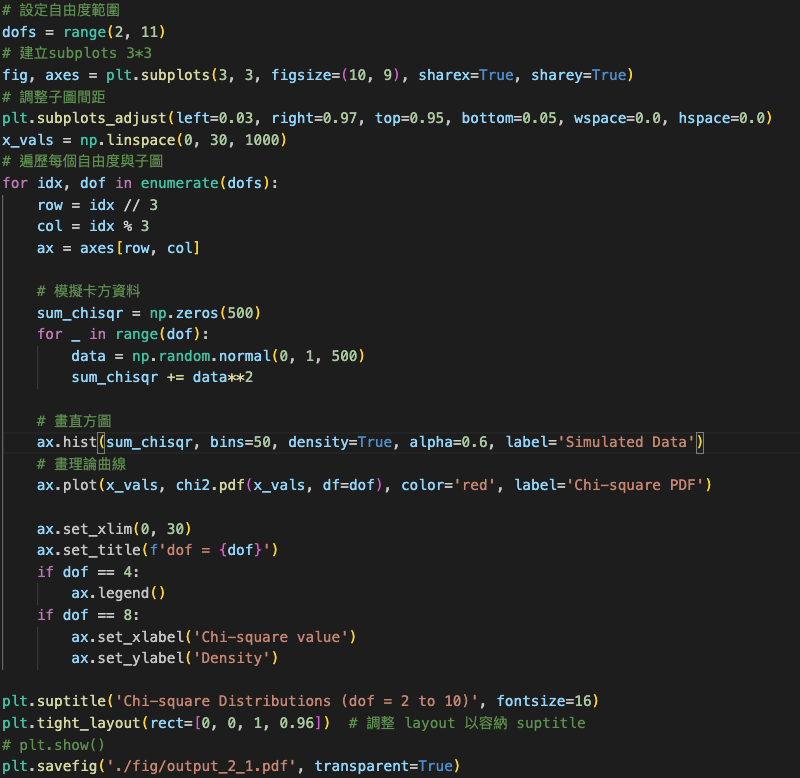
\includegraphics[width=1\linewidth]{figures/code/code_2_5.png}
        \caption{Compare the histogram with the chi-square distribution with different degrees of freedom.}
        \label{fig:code_2_5}
    \end{figure}
\end{enumerate}


\clearpage
\section{實驗數據與分析}
\hfill

\subsection{Practice 1}

\begin{figure}[h]
    \centering
    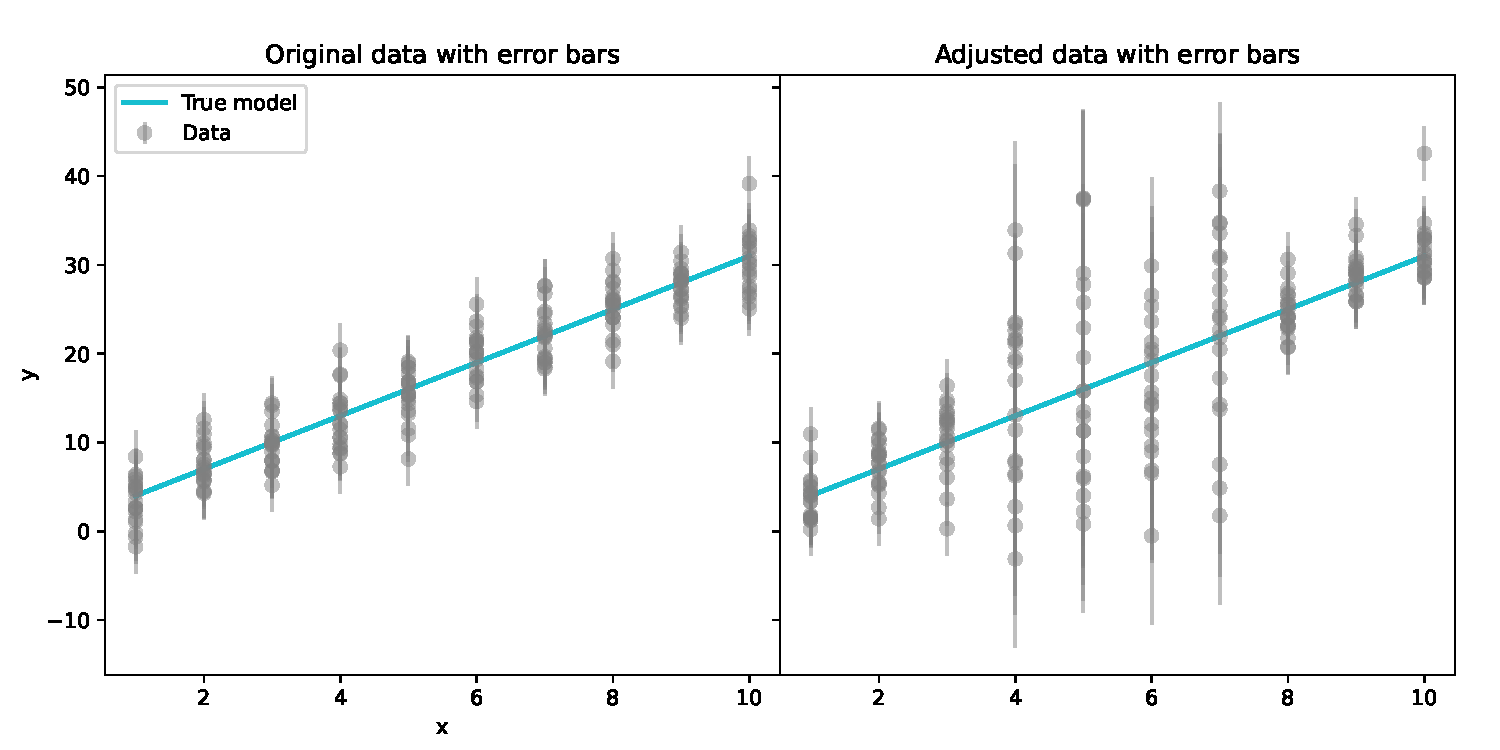
\includegraphics[width=1\linewidth]{figures/output/output_1_1.pdf}
    \caption{Comparison between the original and $\sigma_0$-adjusted $y$ data points.(\textit{left}: Original data with $\sigma_0=3$; \textit{right}: The same with the left panel except for $x=4-7$, where the $\sigma_0$ are changed to 10.)}
    \label{fig:output_1_1}
\end{figure}

The 20 sets of data points defined by a function \(y = mx + k + noise\) with \texttt{x = linespace(1, 10, 10)} are plotted altogether in the Fig.\ref{fig:output_1_1}. As Fig. \ref{fig:output_1_1} shows, the error bars of $x=4-7$ on the \textit{right panel} are significantly enhanced due to the manually changed noise $\sigma_0$ from 3 to 10. This result looks ideal. 
Additionally, Table. \ref{tab:mean_std} lists the mean and standard deviation of the synthetic datasets, denoted as $\mu_{data}$ and $\sigma_{data}$, respectively, compared to the actual model \(y = mx+k\) and the given gaussian noise $\sigma_0$. The discrepancy between the mean and the model, $\Delta$, and the error percentage between $\sigma_0$ and $\sigma_{data}$ are also combined in the Table. \ref{tab:mean_std}. 

In the Table. \ref{tab:mean_std}, the discrepancy $\Delta$ between the model $y=mx+k$ and the $\mu_{data}$ are generally larger if $x=4\sim7$ (bold text in the table), where the $\sigma_0$ is set to be 10. This may be due to the small size of the data set, recalling the law of large numbers (LNN). The sample size of each $x$ is merely 20, in which some of the largely biased data points can still influence the $\mu_{data}$. This reason can also be applied to the cause of the arbitrary and random large error between $\sigma_0$ and $\sigma_{data}$ at some $x$ (e.g., $ x=3, 6, 9$).

\clearpage
\begin{table}[h]
\centering
\caption{The $\mu$ and $\sigma$ of the data compared to the ideal $y$ and given $\sigma_0$}
\vspace{0.5cm}
\large{
\begin{tabular}{c||cc:c|cc:c}
$x$ &   $y=mx+k$    &   $\mu_{data}$  & $\Delta$   & $\sigma_{0}$  &   $\sigma_{data}$ &   error(\%)\\
\hline\hline
1   &   4   &   3.731   &   $-$0.269  &   3   &   2.572   &   14.27\\
2   &   7   &   7.510   &   +0.510  &   3   &   2.706   &   9.80\\
3   &   10  &   10.622  &   +0.622  &   3   &   3.810   &   27.00\\\hline
\textbf{4}   &   \textbf{13}  &   \textbf{15.388}  &   \textbf{+2.388} &   \textbf{10}  &   \textbf{9.850}  &   \textbf{1.50}\\
\textbf{5}   &   \textbf{16}  &   \textbf{17.271}  &   \textbf{+1.271}  &   \textbf{10}  &   \textbf{11.601} &   \textbf{16.01}\\
\textbf{6}   &   \textbf{19}  &   \textbf{15.907}  &   \textbf{$-$3.093} &   \textbf{10}  &   \textbf{7.449}  &   \textbf{25.51}\\
\textbf{7}   &   \textbf{22}  &   \textbf{22.852}  &   \textbf{+0.852}  &   \textbf{10}  &   \textbf{10.067} &   \textbf{0.67}\\\hline
8   &   25  &   24.728  &   $-$0.272  &   3   &   2.488   &   17.07\\
9   &   28  &   28.933  &   +0.933  &   3   &   2.232   &   25.60\\
10  &   31  &   31.625  &   +0.625  &   3   &   3.110   &   3.67
\end{tabular}
}
\label{tab:mean_std}
\end{table}


Fig. \ref{fig:output_1_2} shows the least-square and chi-square fitting results using \texttt{curve\_fit}, including the best-fit curve (dashed line) and the uncertainties (shaded area) of each fitting method. The detailed values of the best-fit parameters are listed in the Table. \ref{tab:mean_std}. (chi-square and least-square fitting are called $\chi^2$ and LS fitting, hereafter)

As shown in the Table. \ref{tab:mean_std}, the best-fit parameters of the two fitting methods, $\chi^2$ and LS fitting, $m$ and $k$, are near the ones of the true model ($m=1$ and $k=1$). The best-fit curves also share the same results in Fig. \ref{fig:output_1_2} as the $\chi^2$ fitting (purple dashed line) and LS fitting (orange dashed line) overlap the true model (cyan solid line). The $\chi^2$ values and the reduced $\chi^2$ in the Table. \ref{tab:mean_std} demonstrates that there is not much deviation between the two fitting methods regarding the values of parameters. 

However, there is a significant dissimilarity in the uncertainties of the two parameters $\Delta m$ and $\Delta k$ between the two fitting methods, $\chi^2$ and LS fitting. The uncertainties of the $\chi^2$ fitting are roughly 2 times smaller than those of the LS fitting.  This is rooted in the fundamental difference between the two methods: the $\chi^2$ fitting weights the sum of the least-squares with the uncertainties of each experiment. In our case, the enhanced uncertainties at $x=4\sim7$ decrease those terms' significance and lessen the covariance matrix's diagonal terms when performing the $\chi^2$ method. At the same time, the LS fitting doesn't consider the experimental uncertainties.

\begin{table}[h]
\centering
\caption{Best-fit parameters of the chi-square and least-square fitting}
\vspace{0.5cm}
\large{
\begin{tabular}{c||c c:c}
Best-fit        &   $\chi^2$ fitting      &   LS fitting    &   True model\\\hline\hline
$m$             &   3.037   &   2.985   &   3\\
$\Delta m$      &   0.076   &   0.167   &   --\\
$k$             &   1.156   &   1.438   &   1\\
$\Delta k$      &   0.495   &   1.037   &   --\\
$\chi^2$        &   0.488   &   0.447   &   --\\
$\chi_{\nu}^2$  &   0.061   &   0.056   &   --
\end{tabular}
}
\label{tab:best_fit}
\end{table}
\clearpage
Despite the uncertainty difference, the shaded area (uncertainties) of the two fitting methods in Fig. \ref{fig:output_1_2} both involve the true model, reassuring that in our data set, there is not a notable contrast between the $\chi^2$ and LS fitting.

\begin{figure}[h]
    \centering
    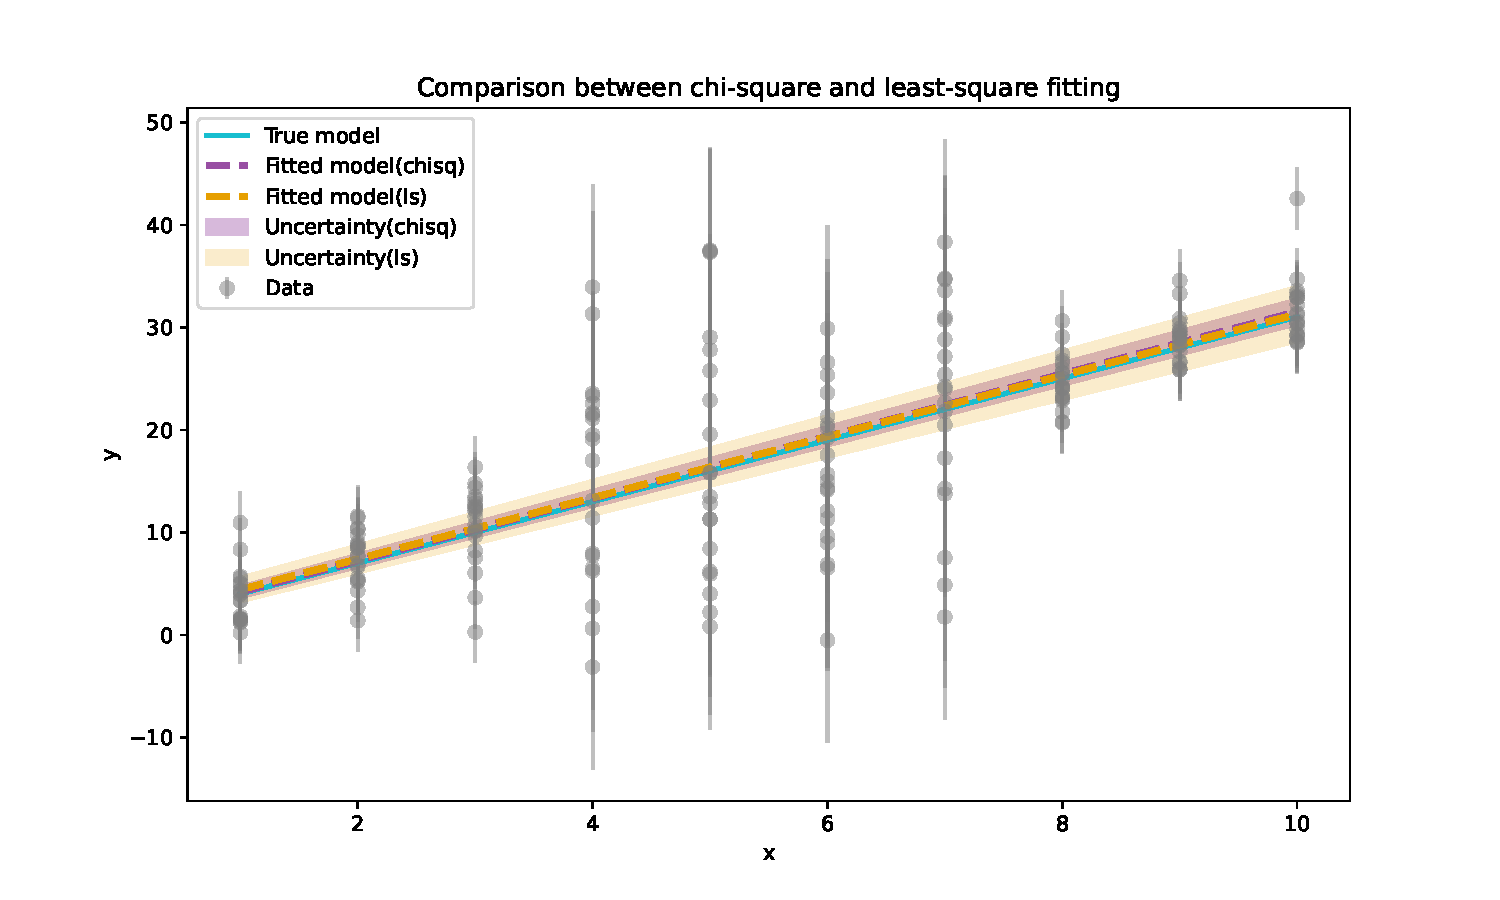
\includegraphics[width=1\linewidth]{figures/output/output_1_2.pdf}
    \caption{Comparison between least-square fitting and chi-square fitting.}
    \label{fig:output_1_2}
\end{figure}



\clearpage
\subsection{Practice 2}
\hfill

The chi-square distribution ($\chi^2$-distribution) is a special case of the gamma distribution, widely used in statistics, especially in hypothesis testing and confidence interval estimation for variance. It describes the distribution of the sum of the squares of $k$ independent standard normal random variables.

There are some properties about the probability density function (PDF) of the chi-square distribution (Eq. \ref{eq:pdf}):
\begin{itemize}
    \item The mean $\mu$ is equal to the degrees of freedom (dof; $k$)
    \item For small $k$, it is highly right-skewed.
    \item As $k\rightarrow\infty$, it approaches a normal distribution via the central limit theorem.
\end{itemize}

In our practice, we generate a 1-d array with 500 elements, which are sampled from a normal distribution with mean = 0 and standard deviation = 1, calculate the chi-square value of each data point, and plot this $\chi^2$ value to histograms. Moreover, we overlap the ideal PDF of the chi-square distribution onto those histograms to compare the two.


\begin{figure}[h]
    \centering
    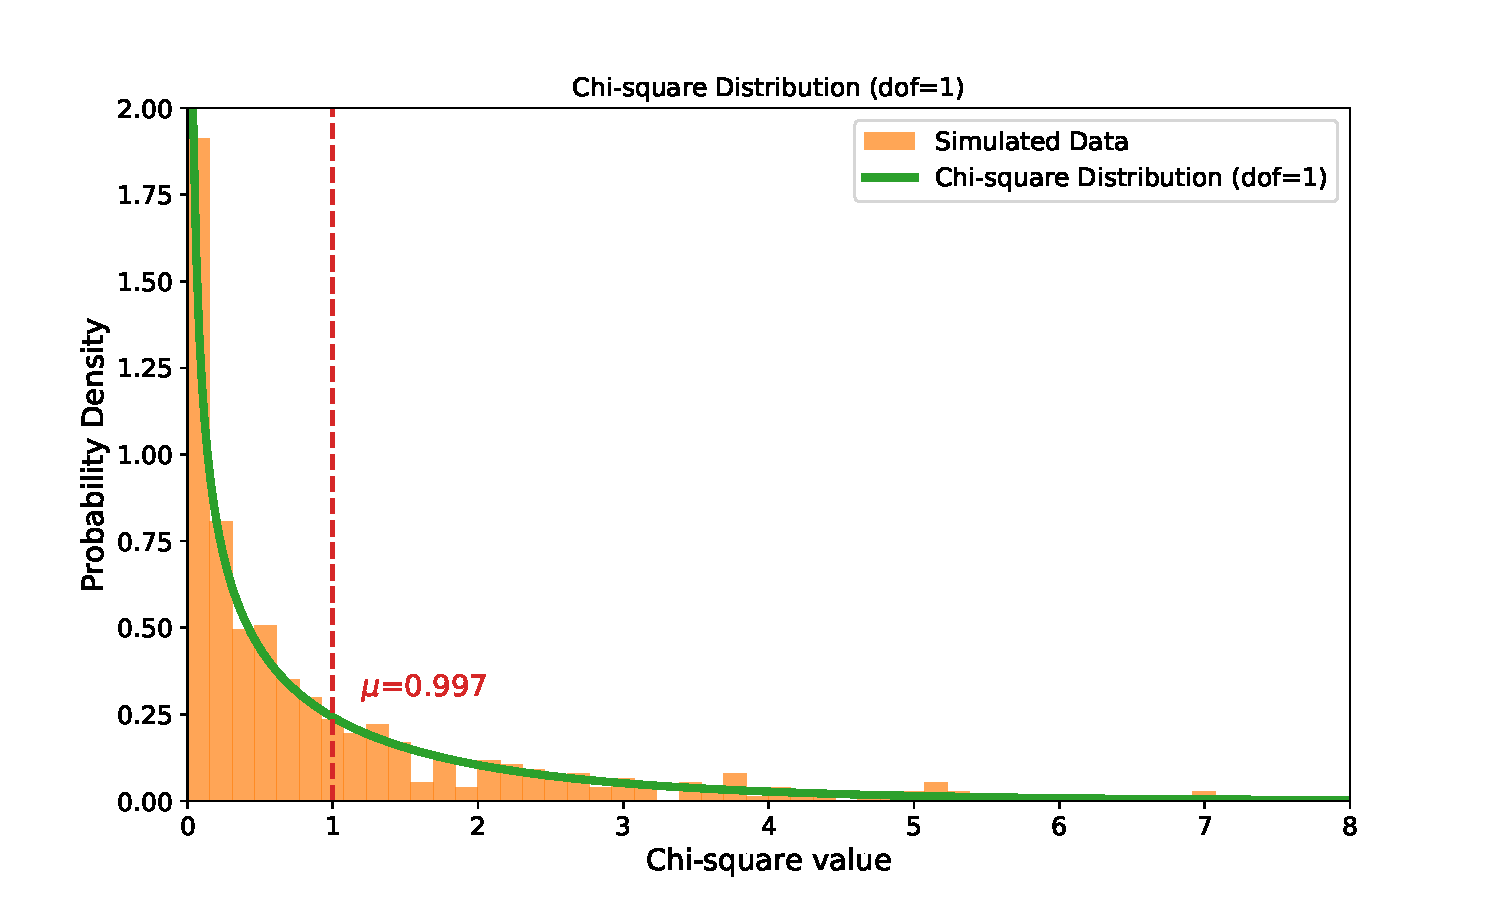
\includegraphics[width=1\linewidth]{figures/output/output_2_1.pdf}
    \caption{Histogram of the calculated chi-square values of the 500 elements with comparison of chi-square distribution with the degrees of freedom = 1}
    \label{fig:output_2_1}
\end{figure}

In Fig. \ref{fig:output_2_1} and \ref{fig:output_2_2}, the chi-square distributions of the generated arrays with dof from 1 to 10 are showcased. When dof = 1 and 2, the $\chi^2$ distribution and the PDF are highly left-skewed, while as the dof are larger, the distributions become less skewed and closer to a normal distribution, matching the abovementioned properties. 

\clearpage
Moreover, the means $\mu$ of the chi-square distributions are in red on Fig. \ref{fig:output_2_1} and \ref{fig:output_2_2}. As a result, the means are around the same as the degrees of freedom. This also goes with the characteristic of the PDF of the chi-square distribution.

\begin{figure}[h]
    \centering
    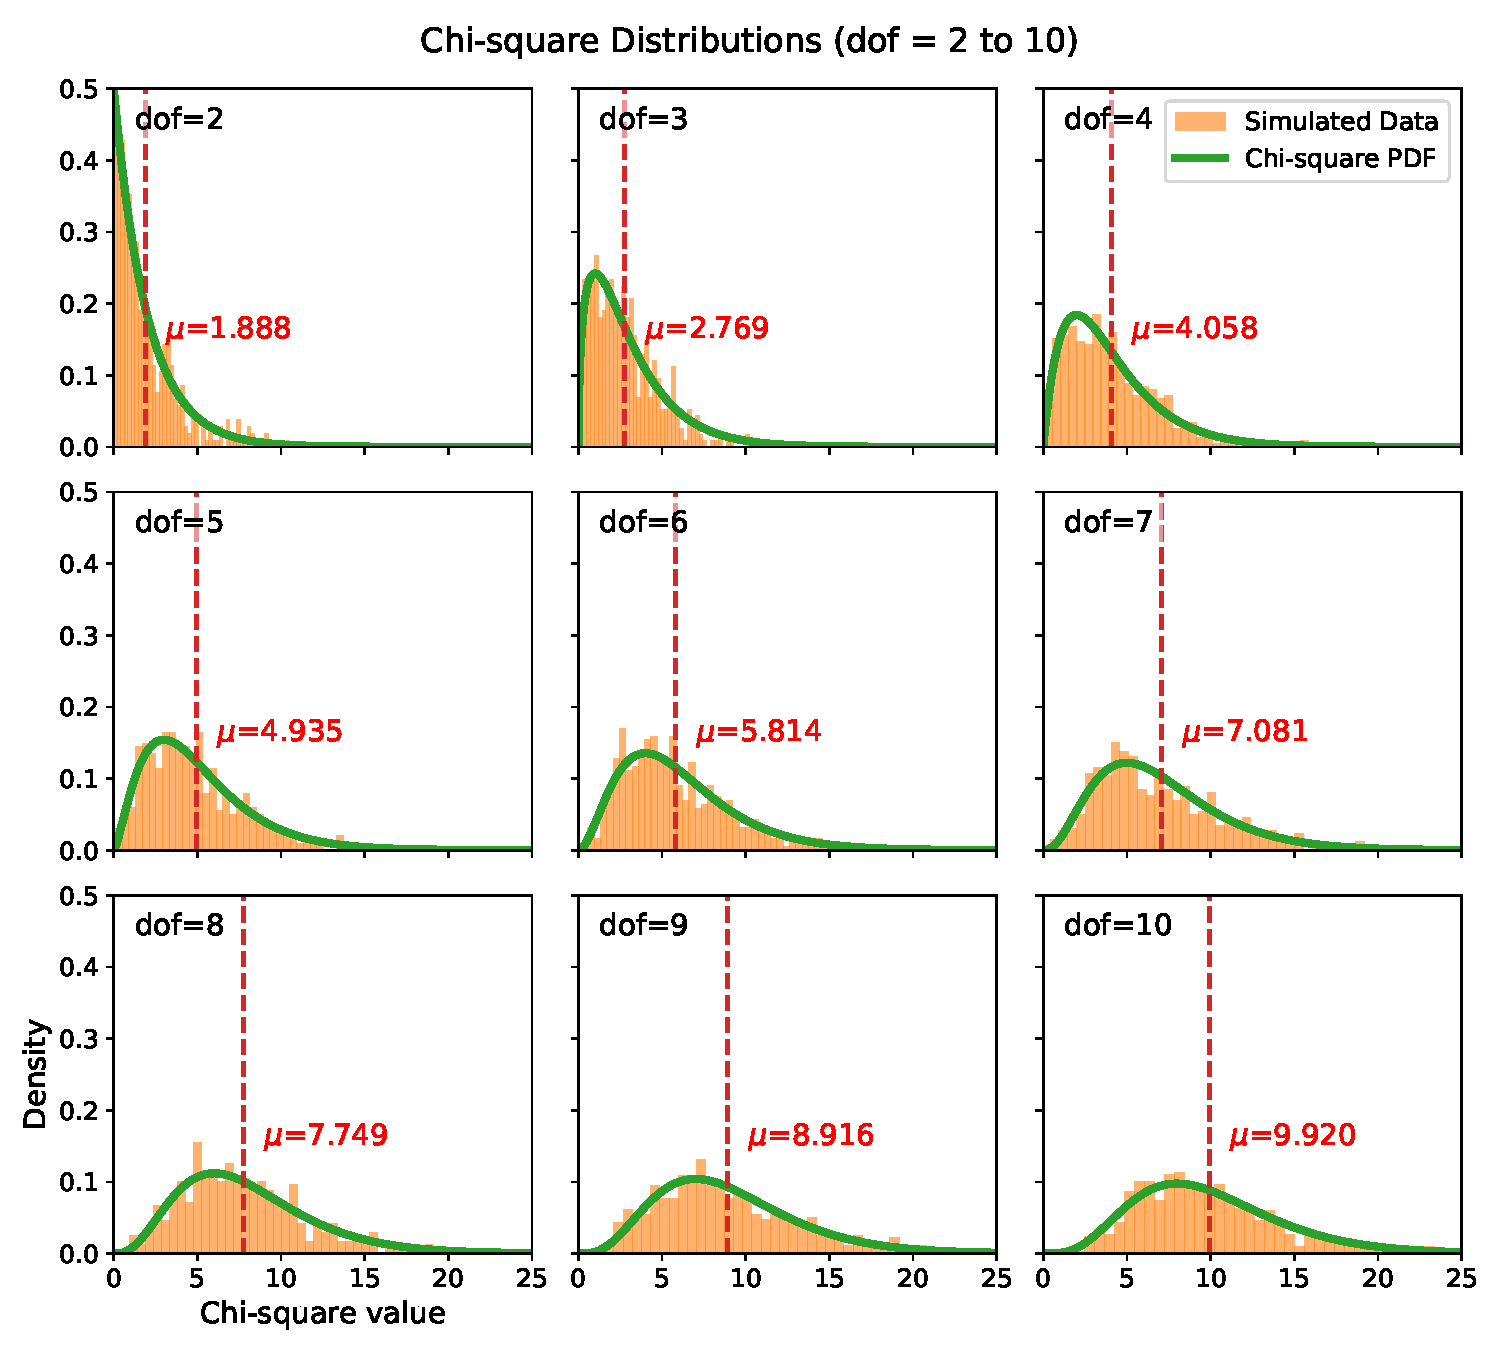
\includegraphics[width=1\linewidth]{figures/output/output_2_2.pdf}
    \caption{Histograms of the calculated chi-square values of the 500 elements with comparison of chi-square distribution with the degree of freedom from 2 to 10 (from top to bottom and left to right).}
    \label{fig:output_2_2}
\end{figure}




\clearpage
\section{問題討論}

\subsection{Practice 1}

\subsubsection{Which fitting method is better in this case? State the reason.}
\hfill

從先前的練習可以知道透過比較$\chi^2_\nu$可判斷擬合結果的好壞,依據如下:
\begin{itemize}
    \item $\chi^2_\nu\approx1$:符合預期
    \item $\chi^2_\nu\ll1$:過度擬合
    \item $\chi^2_\nu \gg1$:欠擬合
\end{itemize}
Table.\ref{tab:best_fit}中,可見$\chi^2_{LS}=0.488$,而$\chi^2_{chi}=0.447$;又本次實驗共生成10個數據,其自由度為:
\begin{equation}
    \nu = 10-2=8
    \nonumber
\end{equation}
可得:
\begin{itemize}
    \item $LS\ fitting$:$\chi^2_\nu=\frac{0.488}{8}=0.061$
    \item $chi\ fitting$:
    $\chi^2_\nu=\frac{0.447}{8}\approx0.056$
\end{itemize}

觀察結果可見,$LS \ fitting$之$\chi^2_\nu$較接近1,理論上為擬合效果較好的方式,這並不符合我們的預期結果,我們所期望的應是由有加入權重的$chi\ fitting$擬合程度較佳;造成此結果我們認為並非$LS\ fitting$真的較為精準,而是由於數據、參數等等皆由電腦所生成,不是真正的實驗數據,導致擬合結果「過度準確」;可由兩者的$\chi^2_\nu$皆遠小於1來佐證。

我們亦可由 Fig.\ref{fig:output_1_2}觀察到$LS\ fitting$所估的參數不確定性明顯大於$chi\ fitting$,表示在考慮誤差大小的情況下,$chi\ fitting$能提供更穩定的參數估計,進一步說明其為更精準的擬合方法。

\subsection{Practice 2}

\subsubsection{What do you find?}
\hfill

藉由Fig.\ref{fig:output_2_2}可見,在$\nu>2$後,當自由度增加時,$\chi^2$的機率密度函數之峰值會向右移,且分佈形狀逐漸平滑;而在Fig.\ref{fig:output_2_1}和\ref{fig:output_2_2}觀察出當自由度等於1、2時,$\chi^2$之PDF在$x \to 0$時發散,整體趨勢類似為exponential decay;所以透過自由度低較不接近常態分佈的觀察可推測出:當自由度較少時,其$\chi^2_\nu$數值的變動會比較敏感。\\($Hint:\ $$\nu=\ $數據量$\ -\ $擬合所使用的參數)

\clearpage

\subsubsection{Considering your previous work on chi-square fitting, describe the relation between those $\mu$, $\sigma$, elements, and the fitting process.}
\hfill

\noindent ($Hint:\mu$為平均數、$\sigma$為標準差)
\\

$\chi^2$計算公式如下:
\begin{equation}
    \chi^2=\sum_i^N(\frac{(y_i-F(x_i))}{\sigma_i})^2
    \nonumber
\end{equation}
其中,$y_i$為實驗數據(在本實驗由電腦生成),$F(x_i)$為模型擬合之數據,$\sigma_i$為每個數據的不確定性。

由於我們的數據點是從常態分佈產生的,則有以下性質:
\begin{itemize}
    \item $\mu$和$\sigma$個別描述資料的中心與其分散程度
    \item 計算$\chi^2$時,$\mu$可等效為期望值,$\sigma$則表示成數據誤差的權重
    \item normalization的公式為:
    \begin{equation}
        x_{normalized}=\frac{x-\mu}{\sigma}
        \nonumber
    \end{equation}
    意義為衡量該數據偏離常態的程度
\end{itemize}

接著根據$practice\ 1$的結果,實際在進行曲線擬合時,可發現若資料點之$\sigma$不同,$chi\ fitting$將進行加權擬合;將誤差大的數據($\sigma$較大)透過計算使其對於$\chi^2$值的貢獻較低,反之則反;而如果我們沒有對數據進行加權擬合的話,其結果等效為$LS\ fitting$。

最後,根據$practice\ 2$的結果,可見$\chi^2$和自由度($\nu$)存在一定關係;欲判斷擬合結果好壞,將仰賴於其比值:
\begin{equation}
    \chi^2_\nu=\frac{\chi^2}{\nu}
    \nonumber
\end{equation}
判斷依據參考4.1.1。

%%%%%%%%%%%%%%%%
\section{總結}
\hfill

實驗中分析了least-square fitting 和 chi-square fitting在具有不同不確定度數據時的差異。Practice 1為了模擬非均勻不確定度,調整了noise的標準差在數據集的數值,並且分別用least square fitting 和 chi-square fitting進行擬合。從結果比較可以看出,非均勻的不確定度對於擬合參數有影響。與least square fitting相比,chi-square fitting對變化的不確定度有更明顯的反應,因此能得出chi-square fitting更適用於具有不均勻不確定度的數據,此外延續前面幾次的實驗,這次也使用reduced $\chi^2$來判斷擬合程度的好壞。Least-square fitting的reduced $\chi^2$值≈0.056,Chi-square fitting的reduced $\chi^2$值≈0.061,擬合結果都遠小於理論值(reduced $\chi^2$≈1),但卡方擬合的數值更接近1,表示其結果較符合預期。得出在error bar變化較大的時候,透過chi-square fitting能得到更準確的擬合結果。Practice 2中,實驗結果之$\chi^2$ 值與理論值接近,可推測出自由度會影響卡方分布的趨勢變化。



\section{分工}
\begin{itemize}
    \item 洪瑜: 問題討論
    \item 黃巧涵: 摘要、前言、總結、分工
    \item 洪懌平: 實驗步驟、實驗數據與分析
\end{itemize}

\section{Appendix}

\subsection{Source code}

\begin{itemize}
    \item \url{https://github.com/hyp0515/exp_phy_ii/tree/main/apr29}
\end{itemize}

%--------------------------------------------------------------%
\end{CJK}
\end{document}